\documentclass[oneside]{book}

\usepackage{mathtools}
\usepackage{graphicx}
\usepackage[utf8]{inputenc}
\usepackage{float}
\usepackage{tabularx}
\usepackage[toc,page]{appendix}
\usepackage{gensymb}
\usepackage{subcaption}
\usepackage{tikz}
\usepackage{circuitikz}
\usepackage{array}
\usepackage{booktabs}
\usepackage{colortbl}
\usepackage{xcolor}
\usepackage{xfrac}
\usepackage{caption}

\usepackage[a4paper, inner=1.5cm, outer=3cm, top=3cm, 
bottom=3cm, bindingoffset=1cm]{geometry} 

\renewcommand{\thesubfigure}{\arabic{subfigure}}


\usepackage{fancyhdr}
\renewcommand{\chaptername}{Experiment}


\begin{document}
\begin{titlepage}

\newcommand{\HRule}{\rule{\linewidth}{0.5mm}} % Defines a new command for the horizontal lines, change thickness here

\center % Center everything on the page
 
%----------------------------------------------------------------------------------------
%	HEADING SECTIONS
%----------------------------------------------------------------------------------------

\includegraphics[width = 50mm]{unitn.jpg}\\[0.5cm]
\textsc{\LARGE Università degli studi di Trento}\\[1cm] % Name of your university/college
\textsc{\Large Group \textbf{MAR01}}\\[0.5cm] % Major heading such as course name

%----------------------------------------------------------------------------------------
%	TITLE SECTION
%----------------------------------------------------------------------------------------

\HRule \\[0.4cm]
{ \huge \bfseries REPORT OF THE EXPERIMENTS\\ PERFORMED IN THE COURSE OF\\[0.3cm] PHYSICS LABORATORY III}\\[0.2cm] % Title of your document
\HRule \\[1.5cm]
 
%----------------------------------------------------------------------------------------
%	AUTHOR SECTION
%----------------------------------------------------------------------------------------

\begin{minipage}{0.4\textwidth}
\begin{flushleft} \large
\emph{Authors:}\\
Canteri Marco\\Biasi Lorenzo\\Luca Vespucci % Your name
\end{flushleft}
\end{minipage}
~
\begin{minipage}{0.4\textwidth}
\begin{flushright} \large
\emph{Professor:} \\
Rolly Grisenti % Supervisor's Name
\end{flushright}
\end{minipage}\\[3cm]

% If you don't want a supervisor, uncomment the two lines below and remove the section above
%\Large \emph{Author:}\\
%John \textsc{Smith}\\[3cm] % Your name

%----------------------------------------------------------------------------------------
%	DATE SECTION
%----------------------------------------------------------------------------------------

{\large \today}\\[3cm] % Date, change the \today to a set date if you want to be precise

%----------------------------------------------------------------------------------------
%	LOGO SECTION
%----------------------------------------------------------------------------------------

%\includegraphics{Logo}\\[1cm] % Include a department/university logo - this will require the graphicx package
 
%----------------------------------------------------------------------------------------

\vfill % Fill the rest of the page with whitespace

\end{titlepage}

\tableofcontents
\chapter{Basic circuits with an operational amplifier}
In this experiment we have built five different circuits. The first is an open loop circuit with the operational amplifier uA741, the goal was to find the maximum voltage output by the op-amp. The last four circuits are in closed loop configuration with a negative feedback, they consist in a follower, a non inverting amplifier, an inverting amplifier and a weighted summing amplifier. We have measured the voltage input and the voltage output of every circut.
\section{Materials}
\begin{itemize}
\item Operational amplifier uA741
\item Resistors, nominal value: 100 $\ohm$, 220 $\ohm$
\item Power supply RIGOL DP831A
\item Waveform generator RIGOL DG1032
\item Multimeter RIGOL DM3068
\item Oscilloscope AGILENT 54261A
\end{itemize}
\section{Experiment setup}
In the first four circuits the output of the waveform generator was a sine wave of 100Hz frequency and a peak-peak voltage of 100mV.
We measured the waveform input signal $v_{in}$ and the output voltage $v_o$ of the op-amp. The measurements were performed using an oscilloscope triggered externally, the signal acquired is an 8 cycles average. The voltage supply of the op-amp was set to $v_{cc} = 15$V for all the circuits.\\
\begin{figure}[H]
\centering
\begin{minipage}{.5\textwidth}
  \centering
  \begin{circuitikz}
 	\draw(0,0) node[op amp,yscale=-1] (opamp) {}
	%(opamp.+) node[left] {$v_+$}
	(opamp.-) ++ (-.3,0) node[ground] {} -- (opamp.-) 
	(opamp.out) node[right] {$v_o$}
	(opamp.up) ++(0,-.5) node[below] {$-v_{cc}$} -- (opamp.up)
	(opamp.down) ++ (0,.5) node[above] {$+v_{cc}$} -- (opamp.down);
	\draw(-3,-1) to[sV] (-3,.5) to[short] (opamp.+);
	\draw(-3,-1) node[ground] {};
	\end{circuitikz}
	\caption{Open loop circuit}
\end{minipage}%
\begin{minipage}{.5\textwidth}
  \centering
  \begin{circuitikz}
 	\draw(0,0) node[op amp,yscale=-1] (opamp) {}
	%(opamp.+) node[left] {$v_+$}
	(opamp.-) ++ (-.3,0) -- (opamp.-) 
	(opamp.-) ++ (-.3,0) -- (-1.5,-1.8) -- (1,-1.8) -- (1,0)
	(opamp.out) node[right] {$v_o$}
	(opamp.up) ++(0,-.5) node[below] {$-v_{cc}$} -- (opamp.up)
	(opamp.down) ++ (0,.5) node[above] {$+v_{cc}$} -- (opamp.down);
	\draw(-3,-1) to[sV] (-3,.5) to[short] (opamp.+);
	\draw(-3,-1) node[ground] {};
	\end{circuitikz}
	\caption{Follower}
\end{minipage}
\end{figure}
\begin{figure}[h]
\centering
\begin{minipage}{.5\textwidth}
  \centering
  \begin{circuitikz}
 \draw(0,0) node[op amp,yscale=-1] (opamp) {}
%(opamp.+) node[left] {$v_+$}
(opamp.-) ++ (-.3,0) -- (opamp.-) 
(opamp.-) ++ (-.3,0) to[R = $R_1$] (-3,-0.5) to (-3,-1) node[ground]{}
(opamp.-) ++ (-.3,0) -- (-1.5,-1.8) to[R,l_=$R_2$] (1,-1.8) -- (1,0)
(opamp.out) node[right] {$v_o$}
(opamp.up) ++(0,-.5) node[below] {$-v_{cc}$} -- (opamp.up)
(opamp.down) ++ (0,.5) node[above] {$+v_{cc}$} -- (opamp.down);
\draw(-4,-1) to[sV] (-4,.5) to[short] (opamp.+);
\draw(-4,-1) node[ground] {};
\end{circuitikz}
\caption{Non inverting amplifier}
\end{minipage}%
\begin{minipage}{.5\textwidth}
  \centering
  \begin{circuitikz}
 \draw(0,0) node[op amp,yscale=-1] (opamp) {}
%(opamp.+) node[left] {$v_+$}
(opamp.-) ++ (-.3,0) -- (opamp.-) 
(opamp.-) ++ (-.3,0) to[R = $R_1$] (-3.4,-0.5) to[sV] (-3.4,-1.7) node[ground]{}
(opamp.-) ++ (-.3,0) -- (-1.5,-1.8) to[R,l_=$R_2$] (1,-1.8) -- (1,0)
(opamp.out) node[right] {$v_o$}
(opamp.up) ++(0,-.5) node[below] {$-v_{cc}$} -- (opamp.up)
(opamp.down) ++ (0,.5) node[above] {$+v_{cc}$} -- (opamp.down);
\draw(-4.3,.5)node[ground] {} to[short] (opamp.+);
\end{circuitikz}
\caption{Inverting amplifier}
\end{minipage}
\end{figure}
For the last circuit we used another sine wave signal with the same 100Hz frequency and a different peak-peak voltage. The oscilloscope's setting and the measurement taken was the same as before.\\The values of the resistor are:  $R_1 =99.89 \pm 0.02$, $R_2 = 218.37\pm 0.04$, $R_3 = 99.89\pm 0.02$ (the measurement were made with the multimeter).
\begin{figure}[H]
\centering
\begin{circuitikz}
\draw(0,0) node[op amp] (opamp) {}
	%(opamp.+) node[left] {$v_+$}
	(opamp.+) ++ (-.3,0) node[ground] {} -- (opamp.+) 
	(opamp.out) node[right] {$v_o$}
	(opamp.down) ++(0,-.5) node[below] {$-v_{cc}$} -- (opamp.down)
	(opamp.up) ++ (0,.5) node[above] {$+v_{cc}$} -- (opamp.up);
	\draw(-5,-1) to[sV] (-5,.5) to[R=$R_3$] (-3,.5) to[short] (opamp.-);
	\draw(-5,-1) node[ground] {};
	\draw(-5,2) to[sV] (-5,3.5) to[R=$R_1$] (-3,3.5) to[short] (-3,.5);
	\draw(-5,2) node[ground] {};
	\draw(-2,.5) to[short](-2,2.2) to[R=$R_2$](1,2.2) to[short](1,0);
\end{circuitikz}
\caption{Weighted summing amplifier}
\end{figure}
\section{Data analysis}
\begin{figure}[H]
\centering
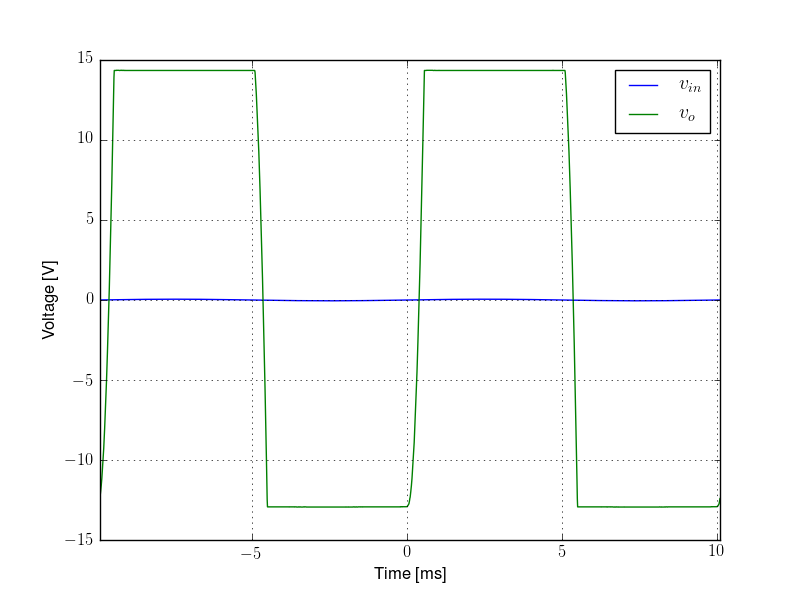
\includegraphics[width=.7\textwidth]{img/scope1.png}
\caption{Open loop configuration}
\end{figure}
In the open loop configuration we get an output (visible in the figure one) that has a max absolute value of $14.35\pm 0.16$\footnote{Error based on oscilloscope's 8 bit resolution} V and a minimum value of $-12.94\pm 0.16^1$ V. In the ideal model we would expect the output to be infinite, as justified from the equation $v_o = A_{ol}(v_+-v_-)$ where $A_{ol}$ tends to infinity. In the physical case the output voltage is costrained by the saturation voltage that's determinated by the voltage applied to the op-amp.
The minimum and maximum value of the output have different absolute value, due to the lack of symmetry between the \emph{npn} and \emph{pnp} trasistors in the final push-pull stage of the op-amp. 
\begin{figure}[H]
\centering
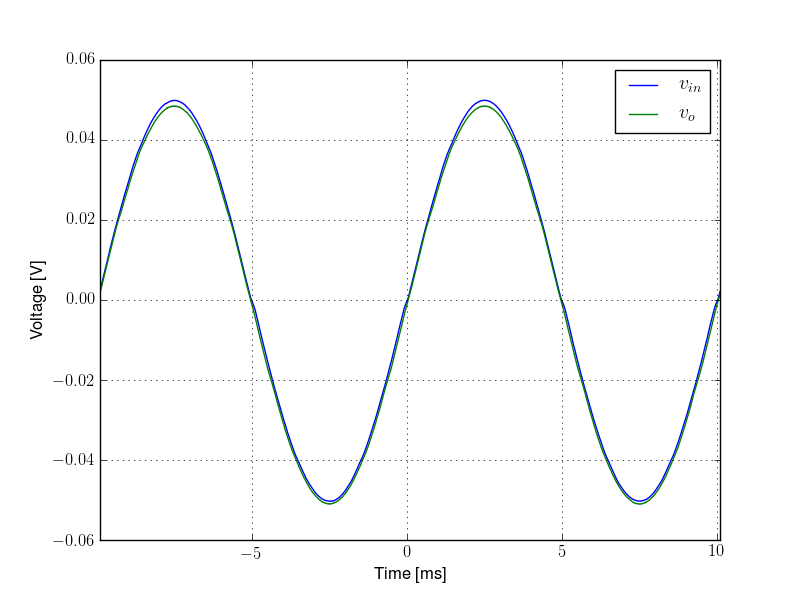
\includegraphics[width=.7\textwidth]{img/scope2.png}
\caption{Emitter follower}
\end{figure}
In the emitter follower we expect, ideally, an output voltage equal to the input one. But we can see in the plot a small discrepancy between the two signals: that is determined probably by the op-amp's offset, as we can see a downward translation in the output, and also by some other non ideal features of the op-amp.
\begin{figure}[H]
\centering
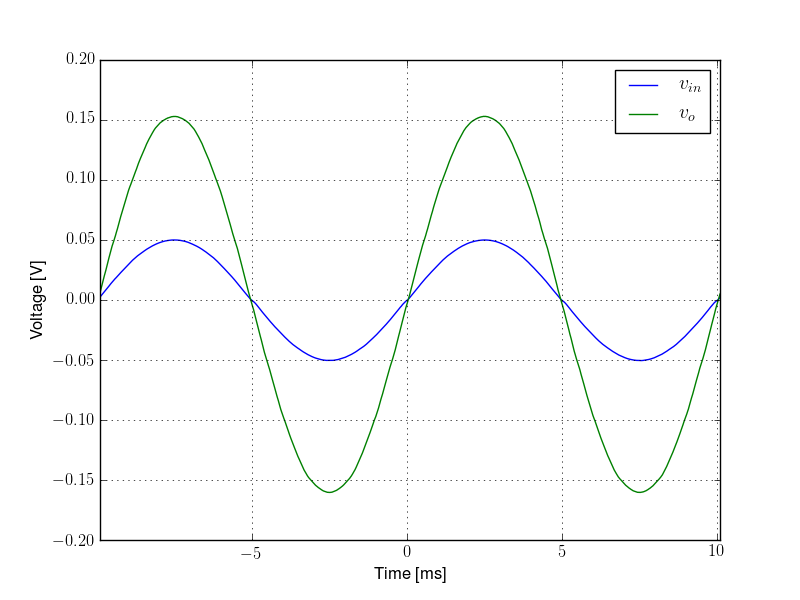
\includegraphics[width=.7\textwidth]{img/scope3.png}
\caption{Non-inverting amplifier}
\end{figure}
In the non-inverting amplifier configuration we expect the output to be: $v_o = v_{in} (1 + \frac{R_2}{R_1})$. The theoretical value calculated using the $v_{in}$ and $R_2$, $R_1$ is $320.3\pm 1.9$ mV. This prediction is not compatible with the output measured $313.4\pm 0.8$, probably because the op-amp is not ideal. 
\begin{figure}[H]
\centering
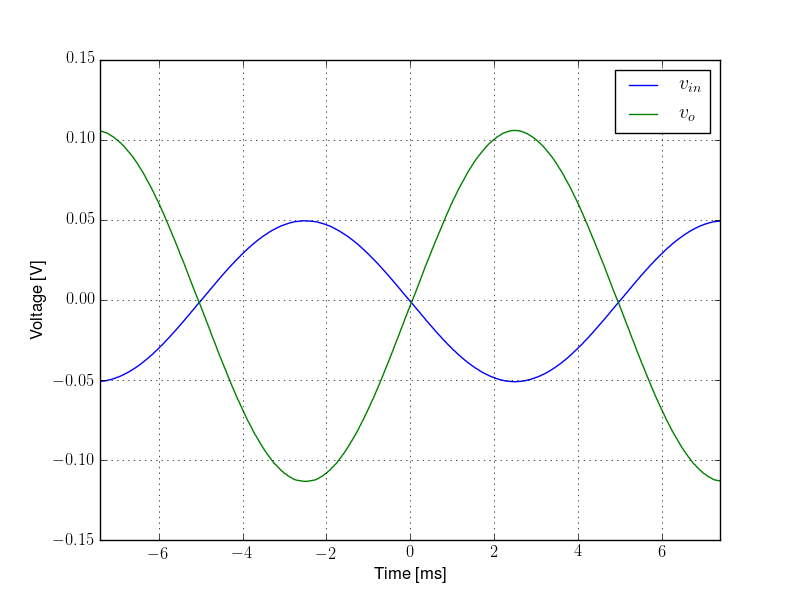
\includegraphics[width=.7\textwidth]{img/scope4.png}
\caption{Inverting amplifier}
\end{figure}
In the circuit x the output should be : $v_o = - v_{in} \frac{R_2}{R_1}$. The pk-pk of the output is $219.4\pm 0.8$ mV that is compatible with theoretical value $219.8\pm 1.9$ mV.
\begin{figure}[H]
\centering
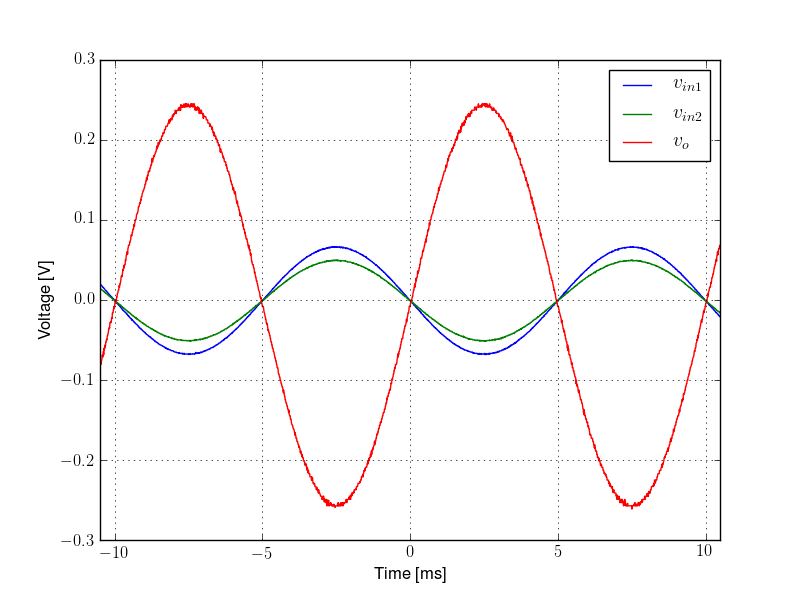
\includegraphics[width=.7\textwidth]{img/scope5.png}
\caption{Weighted summing circuit}
\end{figure}
In the circuit y we used two inputs for aquiring an output voltage. This configuration sums these signals $v_1 = 135.1\pm 0.8$ mV and $v_2 = 101.3\pm 0.8$ mV using the resistors $R_1$ and $R_3$ as weights, giving as output $v_o = - R_2 (\frac{v_1}{R_1} + \frac{v_2}{R_3})$, which gives a pk-pk value of $516.7\pm 2.7$ mV. The theory in this case it's not at all compatible with the measurament $506\pm 0.8$ mV, but that's, most likely, caused by the noise in the output.
\chapter{Let's get more confident with our little friend op-amp}
We designed a non-inverting amplifier with a variable gain by using a trimmer. The second circuit designed was a summing amplifier with an unitary gain. We built a current source generator of $1$mA and tested it with a variable load. We tested the efficacy of the emitter follower configuration in mismatching the source's impedence. Last we designed a differential amplifier with a predetermined gain.
\section{Materials}
\begin{itemize}
\item Operational amplifier uA741
\item Resistors and trimmers
\item Power supply RIGOL DP831A
\item Waveform generator RIGOL DG1032
\item Multimeter RIGOL DM3068
\item Oscilloscope (To be inserted)
\item Two capacitance of nominal value of $100$nF
\end{itemize}
\section{Experiment setup}
In all the circuit we placed two capacitors connecting the op-amp's pins for the power supplying to the ground. This was done with the aim of reducing the noise in the output.
In the current generator we used a DC voltage generator of $x$V and we placed the trimmer in the feedback branch. In all the other circuits we used an input with an amplitude of $1$V and a frequency of $100$Hz.
In the summing amplifier we used resistors $R_1$ $R_2$ and $R_3$ $R_4$ of equal ratio, for obtaining a gain of one.
In the emitter follower test, we first built the circuit in figure X and then the circuit in figure Y and we examined the difference in the output.
In the differential amplifier we first used just one input signal V$1$ and we put to ground the non-inverting input. This way we were able to measure the gain of the circuit. And we built the configuration in figure X using V$1 =$ V$2$ and we tried to get an output equal to $0$ by changing the resistace of the trimmer that is in serie with R$1$.


\end{document} 
\grid
